In this chapter we describe the overall structure digital back-end of the Q-Pix design.
We would like to take a moment here to note here that we refer to each node in the array is implemented as a lattice ice40UP FPGA 

Additionally, this chapter is divided into two parts. 
The first part we give a detailed description of the digital-system, and its requirements to successful in a Q-Pix based detector of DUNE scales.
The motivation here is to outline how the digital backend of Q-Pix based readout fits into the DUNE-FD LArTPC. 
The second part of this chapter is dedicated to the first evaluation boards developed and tested which are implemented in Lattice iCE40UP FGPAs \citep{lattice_ice40up_datasheet}.
The second part outlines the design of the PCB on which these FPGAs are implemented, as well as basic results of these FGPAs, which are motivated from the first part of this chapter.

The Lattice Semiconductor FPGAs \citep{lattice_ice40up_datasheet} were selected because of the small form factor, pin out, availability, as well as lower power consumption.
There are planned tests for future, but not presented here to indicate its viability of over-the-counter FPGAs in LArTPc. 
If such cheap and available FPGAs were shown to be reliable use in a LArTPC environment, that would greatly influence future detector development and selection for Q-Pix.

The vast majority of the work presented in this chapter is my own individual work.

\section{Digital Design Overview}

The digital system of the entire Q-Pix design begins at the electronic collection of a recorded timestamp in respond to a reset-time-difference sent from the analog front-end.
Then, all data that are recorded for each pixel, and the only data required for a full analysis of all reconstruction with a LArTPC are:

\begin{itemize}
    \item 32 bit timestamp
    \item Pixel X location ($\le 4$ bits)
    \item Pixel Y location ($\le 4$ bits)
    \item APA reference number ($\le 4$ bits)
\end{itemize}
\label{bit_calc}

\begin{figure}[]
\centering
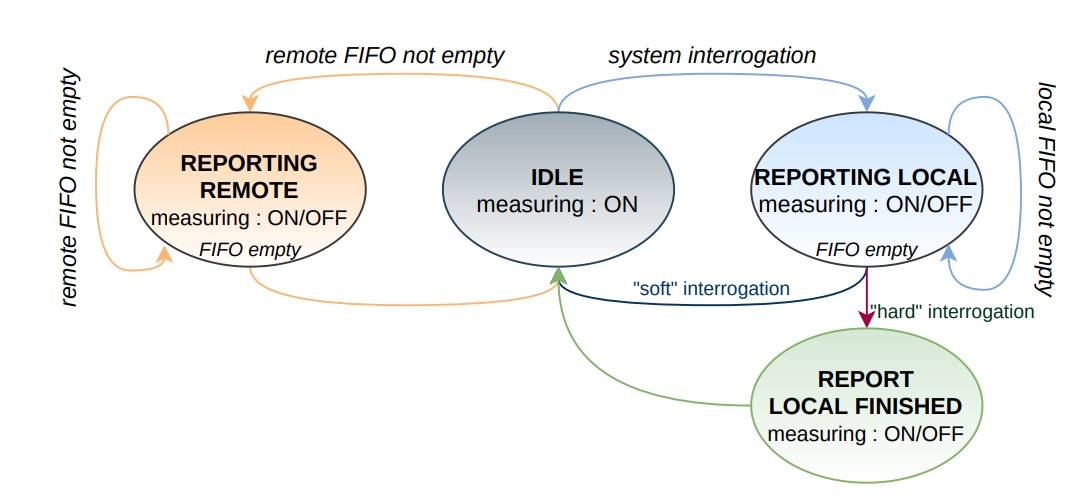
\includegraphics[width=\textwidth]{images/digital_fsm_overview.jpg}
\caption{Diagram of the Digital node's FSM which determines how to respond to incoming packets.}
\end{figure}


\begin{figure}[]
\centering
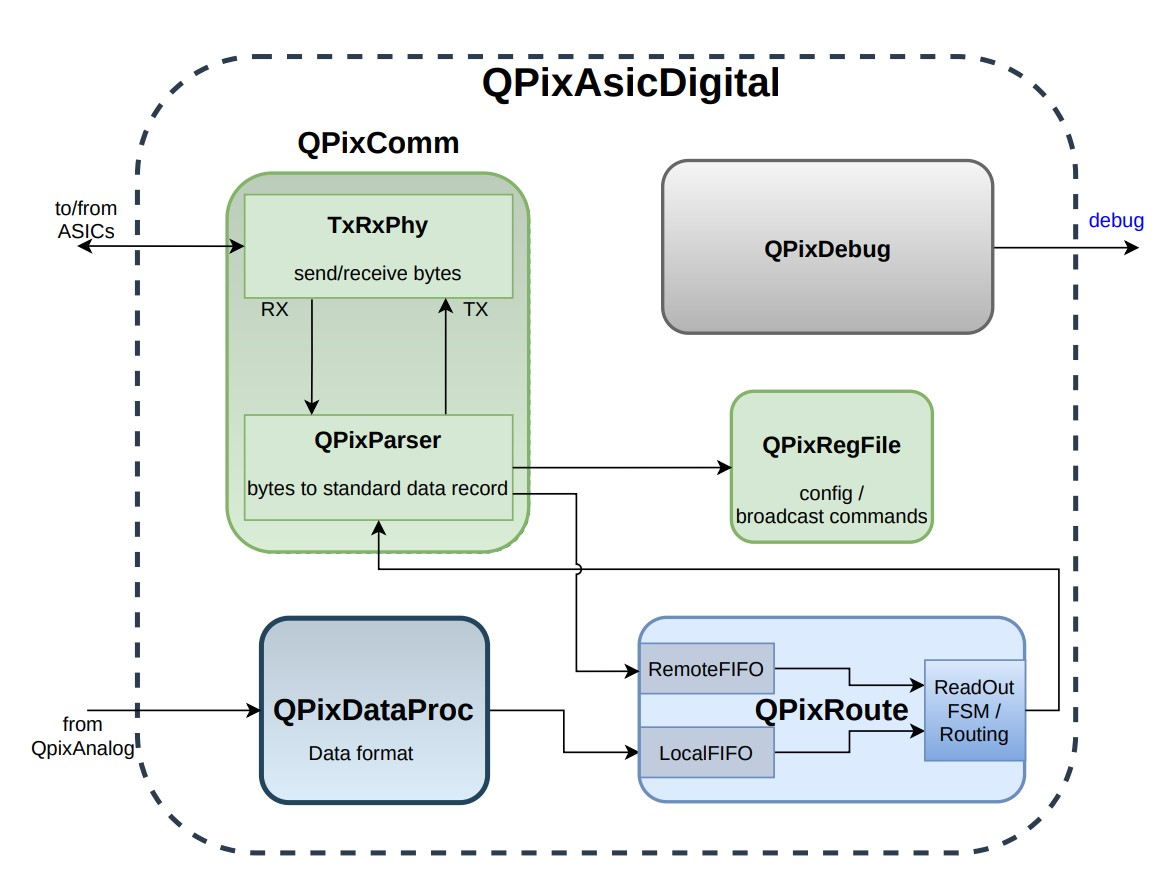
\includegraphics[width=\textwidth]{images/digital_node_overview.jpg}
\caption{Diagram of the Digital node.}
\end{figure}

Each of these remote ASICs are running on free-running independent clocks, with an expected frequency of $\approx$ 30 MHz.

\subsection{Basic System Requirements}

Reset time differences are a function of the accumulated charge compared to the integrating capacitance for this specific pixel.
The sheer number of pixels required for an APA (and the entire module) require an effective means of charge and time calibration, stable buffer depths, and protection against single-point failure (SPF). 

\subsubsection{Charge Calibration of each Pixel}

Natural decay products produced by $^39$Ar provide a continous source of incoming current across a LArTPC.


\subsubsection{Time Calibration of each Node}

\subsubsection{Inter-Node communication via endeavor protocol}
\label{sect:endeavor}


\subsubsection{The Structure of a Data Word}

Each node communicates via an entire packet, which is always 64 bits long. 
The communication protocol~(\ref{sect:endeavor})

\subsubsection{Comments on Data Rates and required Computing}

Based on the minimum number of bits for each RTD \ref{bit_calc} we can calculate minimum data rates for a full APA section and extend to this to 


\section{The Digital Finite State Machine}

The Finite State Machine (FSM) of the remote digital ASIC outlines the designed behavior response to inputs from a controlling DAQ node.

\begin{figure}[]
\centering
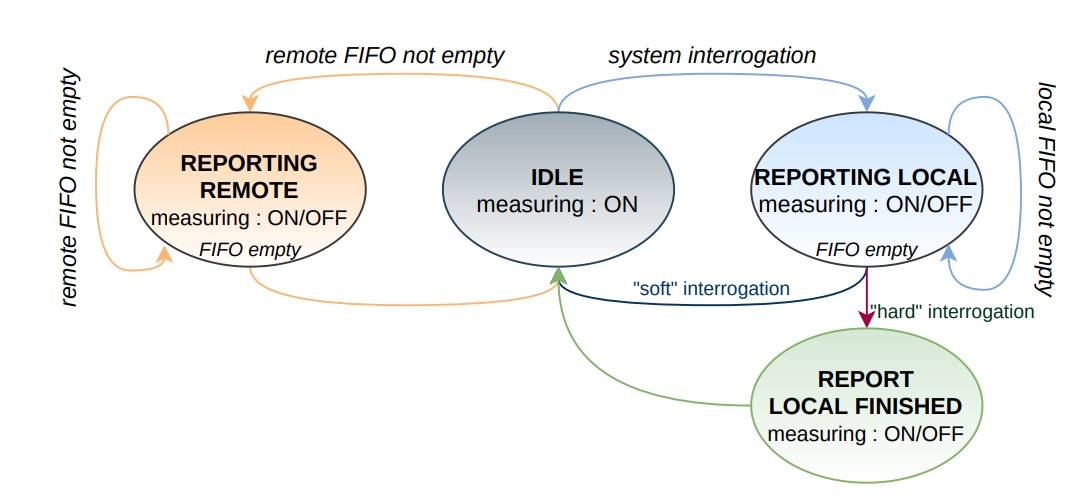
\includegraphics[width=\textwidth]{images/digital_fsm_overview.jpg}
\caption{Overview of the FSM design, courtesy of Vasily Shebalin.}
\end{figure}

\begin{itemize}
    \item Idle, Acquisition State
    \item Transmit Local
    \item Transmit Finish
    \item Transmit Remote
    \item DONE
\end{itemize}
\label{fsm_state_labels}

\section{The Parameter Space of the Digital System}


\subsection{Buffer Depth Requirements}

The required buffer depth of each node in an array is the maximum number of timestamps the node can store in memory before running out of room.

%% QDB Hardware Discussion
\section{QDB Design Overview}

%% schematic of PCB

\section{Power and Current Characteristics}



\section{Timing Stability}

We describe here the methods of measuring a stable time for different configurations of the nodes. 
We also comment on the results of the timing with resepect to the minimum required timing sensitivity in order to have accurate timestamp reconstruction.

\section{Analysis of Systematics for Different System Implementations}

\section{Towards the Integration of a DAQ-Node}

\section{Comments on A Super-DAQ-Node}

Each APA module within a larger DUNE module must ultimately be interconnected so that the entire module can be readout.
As described above, a single modular tile is controlled by an individual DAQ node, where many constitute a complete APA.
Therefore, we refer to the device that digitally multiplexes all of the DAQ node data as the "Super DAQ Node" (SDN).
Then, we imagine the final multiplexing stage for an entire DUNE module as an array of SDNs, each of which consistute an array of DAQ nodes, where each DAQ node is a 2-D array of Q-Pix based ASICs.

The total number of request SDNs within the full dune module depends on the final size of a DAQ-node controlled tile.

\section{Summary}
